\chapter{Planificación}

Como hemos mencionado anteriormente el proyecto va a seguir las prácticas y principios de la metodología ágil. Esta sigue una serie de 17 principios que se pueden consultar en \href{https://agilemanifesto.org/iso/es/manifesto.html}{el manifiesto ágil}. Estos principios se basan en la satisfacción del cliente mediante la entrega temprana y continua de valor poniendo un especial énfasis en la excelencia técnica, en el buen diseño, en la planificación y en la simplicidad.

Para seguir estos principios la memoria ha de realizarse de forma iterativa e incremental, de forma que se vaya realizando conforme se va avanzando y tomando decisiones en el proyecto para estar constantemente describiendo cómo estamos aportando valor al mismo.

Para mejorar el flujo de trabajo y la toma de decisiones, se han empleado herramientas y metodologías basadas en las historias de usuario previamente definidas en \ref{sec:historias-de-usuario}. Esto garantiza la entrega de un producto de calidad que cumpla con los objetivos establecidos.

\section{Metodología utilizada}

En esta sección se van a documentar las diferentes tomas de decisiones que se han llevado a cabo a lo largo del proyecto en cuanto a herramientas y metodologías se refiere para asegurar la excelencia técnica, el buen diseño y la planificación.

\subsection{\textit{Git y GitHub}: control de versiones y colaboración}

Para el control de versiones se ha utilizado \textit{Git}, un sistema de control de versiones que permite llevar un control de los cambios en el código fuente.

Para la colaboración y hospedaje del código fuente se ha usado \textit{GitHub}, una plataforma que permite alojar proyectos de \textit{software} y colaborar en ellos. Dentro de \textit{GitHub} tenemos diferentes funcionalidades que han sido de ayuda para el desarrollo del proyecto.

El repositorio del proyecto se puede encontrar en la siguiente dirección: \url{https://github.com/danigonzser/proyecto-tfg}

\subsubsection{\textit{Issues}}

A lo largo del proyecto se van a ir encontrando diferentes problemas que se han de resolver. Para llevar un control de los mismos se han ido creando \textit{issues}. Estos no solo son descripciones de los problemas que se quieren resolver, sino que pueden ser una buena medida para saber si se progresa hacia el \textit{milestone} o no.

\begin{figure}[H]
    \caption{Captura de pantalla del listado de \textit{issues} del repositorio del proyecto de \textit{GitHub}.}
    \centering
    \vspace*{0.5cm}
    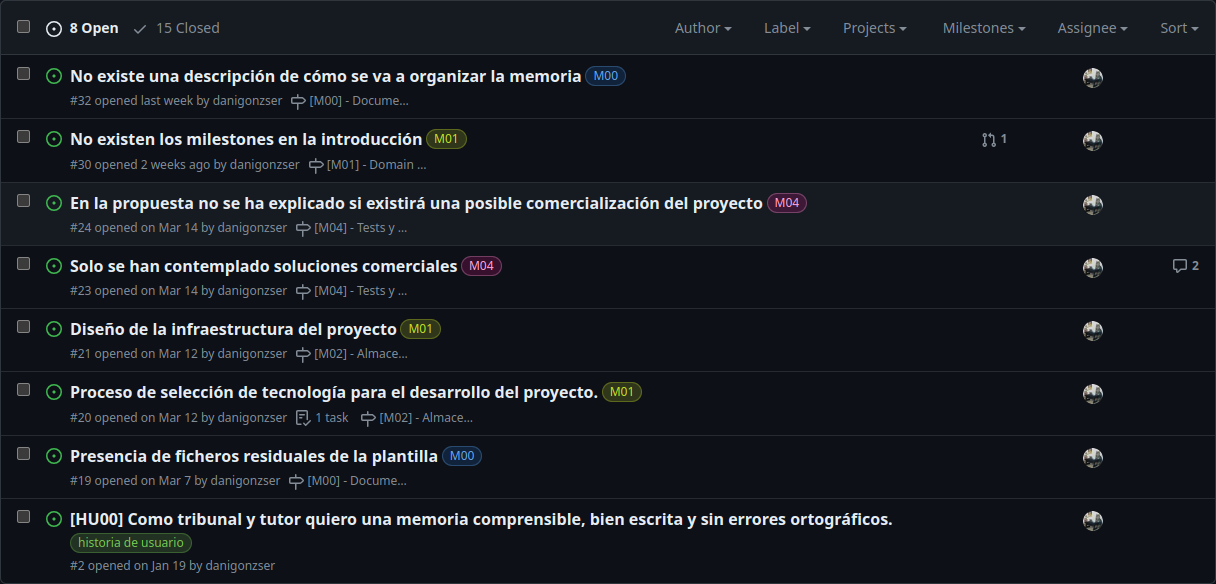
\includegraphics[scale=0.2]{figuras/github_issues.png}
\end{figure}

\subsubsection{Pull requests}

Los pull requests son una forma de proponer cambios en el código fuente sin que estos se apliquen directamente al código fuente o rama principal sin una aprobación previa. Estos son una manera de revisar que los cambios mantengan la excelencia técnica y calidad del proyecto.

Para proteger la rama principal o \textit{master} de cambios no deseados se han configurado una serie de reglas que impiden la integración de cambios a menos que:

\begin{itemize}
    \item Los tests deben de haberse realizado de manera exitosa.
    \item Que la rama esté actualizada.
    \item Que las conversaciones hayan sido resueltas.
\end{itemize}

A continuación se muestra una captura de pantalla de la lista de \textit{pull requests} del proyecto hasta el momento.

\begin{figure}[H]
    \caption{Captura de pantalla del listado de \textit{pull requests} del repositorio del proyecto de \textit{GitHub}.}
    \centering
    \vspace*{0.5cm}
    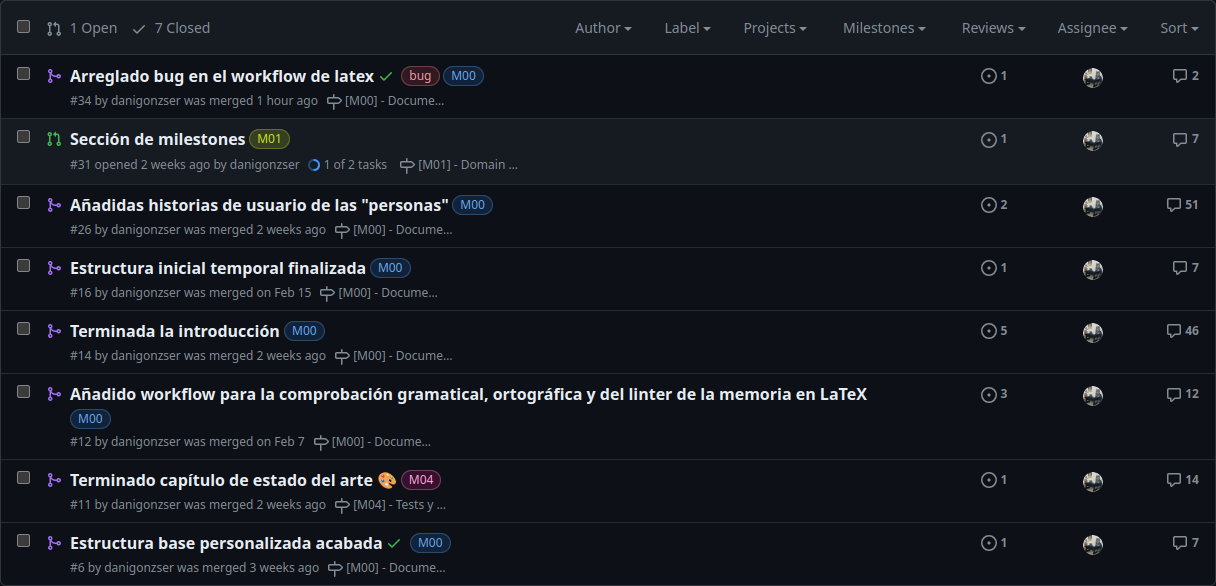
\includegraphics[scale=0.2]{figuras/listado_pull_requests_github.png}
\end{figure}

En la imagen se puede apreciar que se han abierto 8 \textit{pull requests} hasta el momento. Los que están en color morado son los \textit{pull requests} que ya han sido integrados en la rama principal y el que está en color verde es el que todavía no está integrado.

\begin{figure}[H]
    \caption{Captura de pantalla del contenido de una \textit{pull request}.}
    \centering
    \vspace*{0.5cm}
    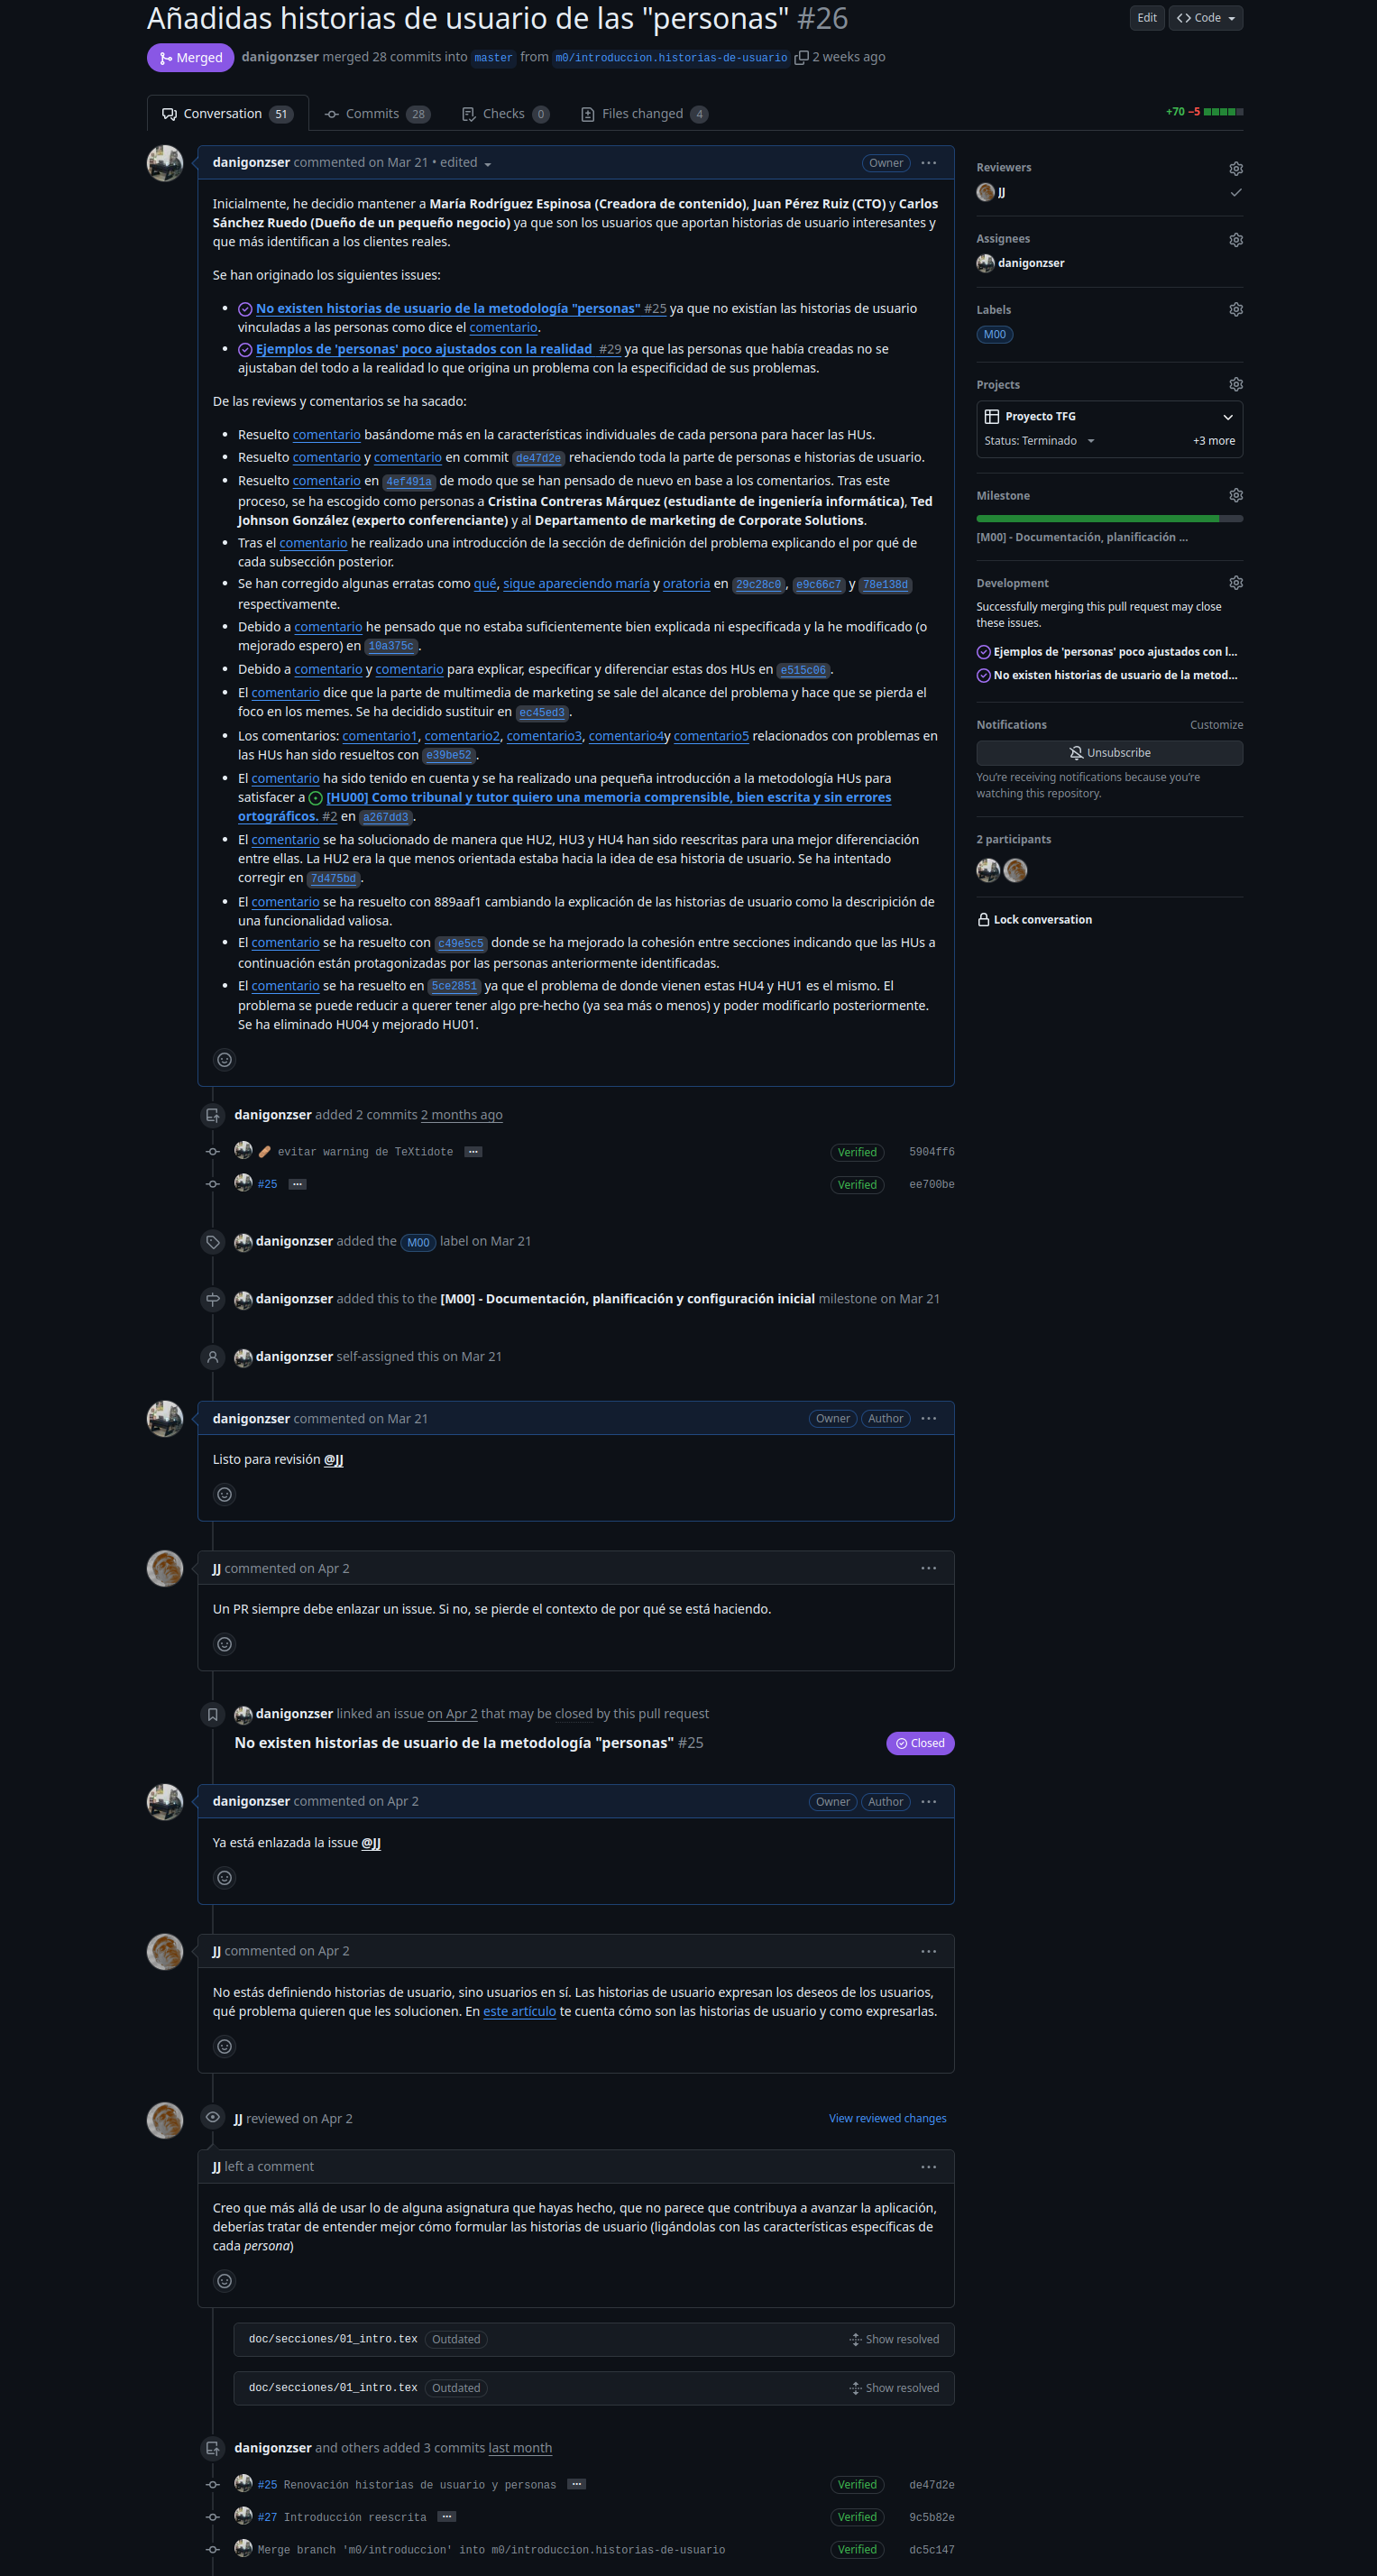
\includegraphics[scale=0.1]{figuras/pull_request_github.png}
    \label{fig:contenido_pull_request}
\end{figure}

Como se puede ver en la figura \ref{fig:contenido_pull_request} el estado de la \textit{pull request} es \textit{merged} lo que significa que ya ha sido integrado en la rama principal. Más abajo se puede ver el cuerpo de la misma donde residen todas las \textit{issues} que han sido creadas y consecuentemente resueltas con esta \textit{pull request}. Más abajo se puede ver el historial de commits y de conversaciones que se han ido originando a lo largo de la resolución. Al final de la imagen es donde podemos ver esas conversaciones que deben ser resueltas antes de integrar los cambios en la rama principal. Finalmente, a la derecha se muestran detalles como el revisor, el asignado, las etiquetas, el proyecto al que pertenece, el \textit{milestone} y las \textit{issues} relacionadas.

\subsubsection{\textit{Projects}: tablero kanban}

La funcionalidad de projects de \textit{GitHub} se ha utilizado para llevar un control de la evolución y progreso de los \textit{issues} y \textit{pull requests}. Se ha implementado un tablero \textit{kanban} como se puede ver en la imagen \ref{fig:tablero_kanban} que permite ver de un vistazo el estado de los \textit{issues} y \textit{pull requests}. Esto es muy útil para saber si se progresa, cómo se están resolviendo los problemas y si se está cumpliendo con los objetivos marcados.

\begin{figure}[H]
    \caption{Captura de pantalla del tablero \textit{kanban} en la sección de \textit{projects} de \textit{GitHub}.}
    \centering
    \vspace*{0.5cm}
    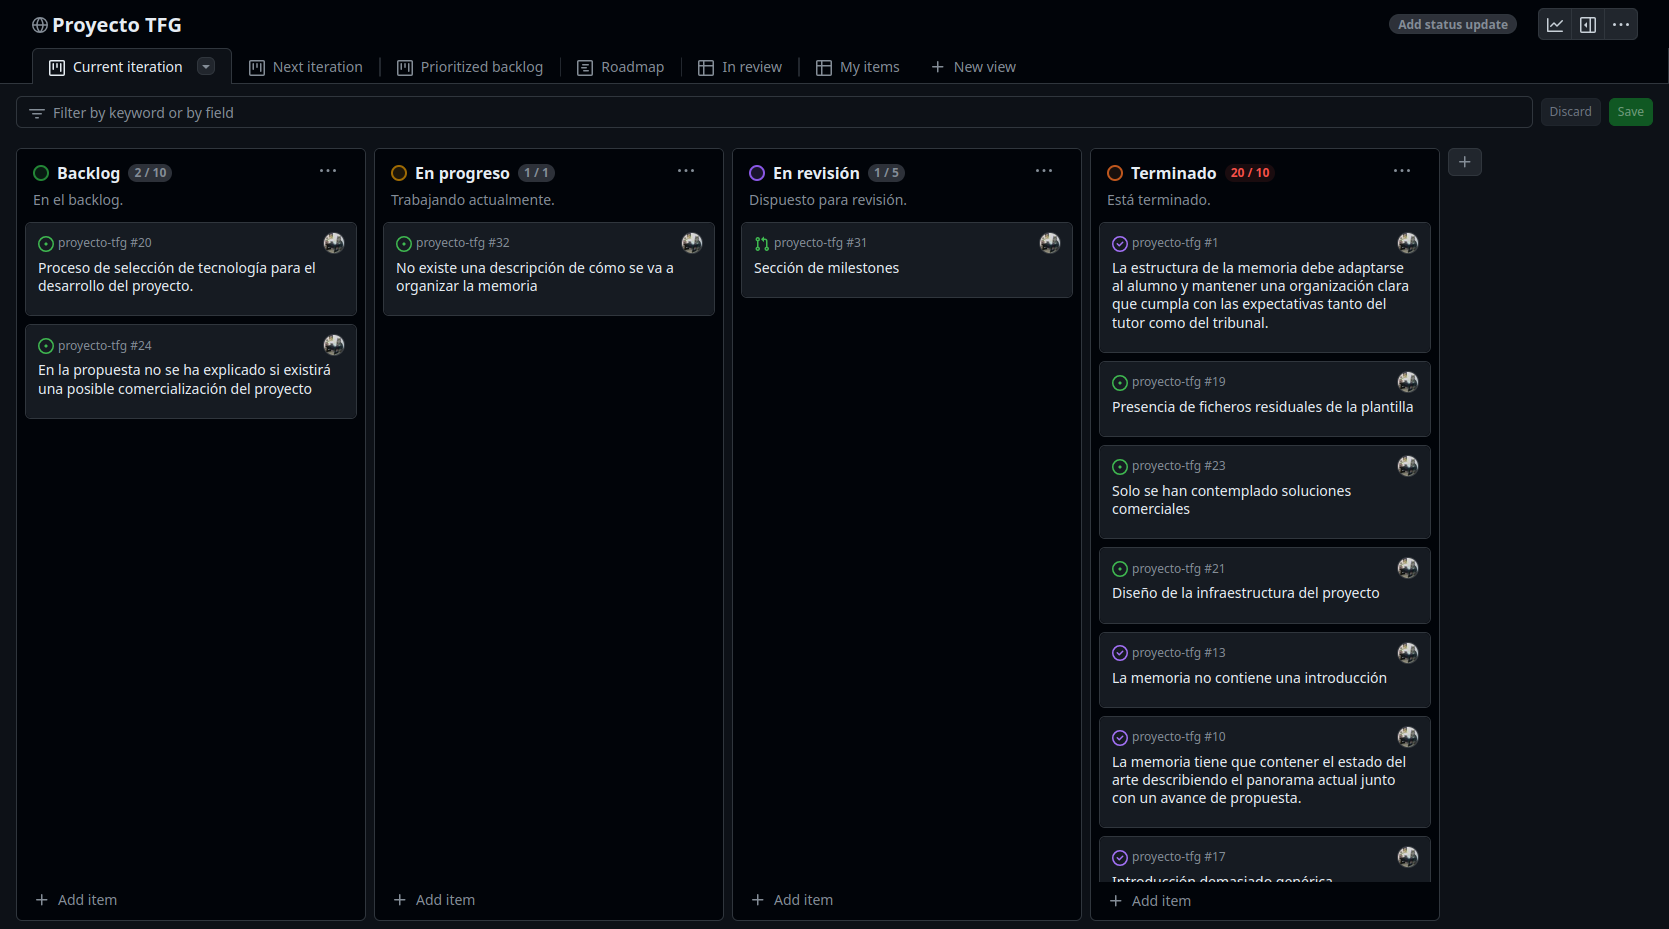
\includegraphics[scale=0.2]{figuras/projects_github.png}
    \label{fig:tablero_kanban}
\end{figure}

\subsection{Documentación del proyecto}

La documentación del proyecto es una de las partes más importantes del trabajo de fin de grado si no la que más por lo que se ha de poner especial atención en que esta sea de calidad y cumpla con los requisitos establecidos por tutor y tribunal. Para dar cuenta de esto, la memoria se ha elaborado en \href{https://www.latex-project.org/}{\LaTeX{}}, un sistema de composición tipográfica de alta calidad; incluye funciones diseñadas para la producción de documentación técnica y científica además de estar disponible como software libre.

Para complementar, comprobar y mejorar la calidad de la documentación se ha usado una serie de herramientas que se han integrado en el flujo de trabajo local tanto con extensiones de (\href{https://code.visualstudio.com/}{Visual Studio Code}) como con herramientas ejecutadas en la linea de comandos.

\subsubsection{Extensión de \textit{Visual Studio Code}: \textit{LaTeX Workshop}}

LaTeX Workshop es una extensión para Visual Studio Code, cuyo objetivo es proporcionar funciones básicas para la composición tipográfica LaTeX con Visual Studio Code. Esta extensión proporciona una serie de características que facilitan la escritura de documentos en LaTeX como la previsualización en tiempo real, la compilación del documento, la visualización de errores y advertencias.

A mayores, esta extensión me ha permitido elegir la receta de compilación que se va a utilizar, la cual se ha configurado para que se compile la memoria junto con la bibliografía.

\begin{figure}[H]
    \caption{Captura de pantalla de \textit{Visual Studio Code} con la extensión \textit{LaTeX Workshop} activada.}
    \centering
    \vspace*{0.5cm}
    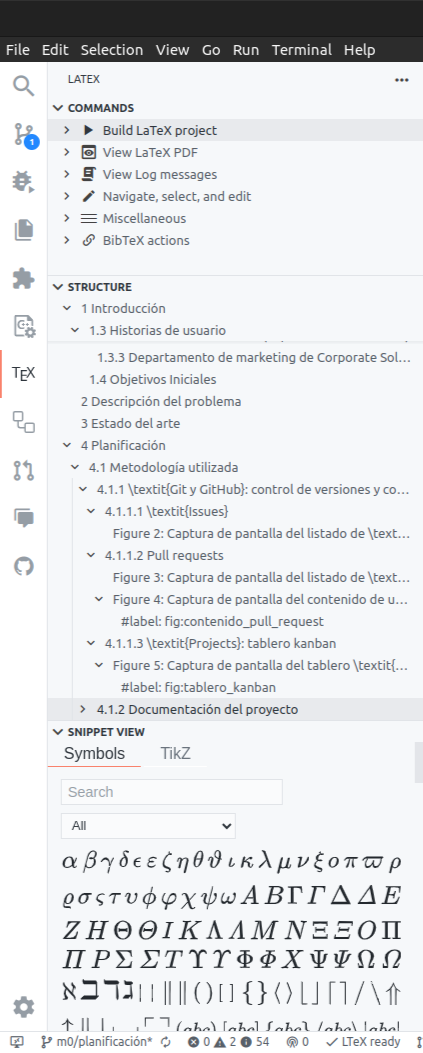
\includegraphics[scale=0.2]{figuras/latex_workshop_extension.png}
    \label{fig:latex_workshop_extension}
\end{figure}

\subsubsection{Extensión de \textit{Visual Studio Code}: \href{https://github.com/valentjn/vscode-ltex}{\textit{LTeX LanguageTool grammar/spell checking}}}

La extensión \( LT_E X \) permite comprobar la gramática y la ortografía de varios lenguajes de marcado en \textit{Visual Studio Code} mediante LanguageTool (véase \ref{sec:languagetool}).

Esta extensión suele trabajar de forma offline teniendo una instancia local de \textit{LanguageTool}, pero en nuestro caso y para mejorar las comprobaciones se ha configurado para que trabaje a través de peticiones HTTP a un contenedor de \textit{Docker} con la imagen \href{https://hub.docker.com/r/erikvl87/languagetool}{erikvl87/languagetool} a modo de servidor. En adición, se ha añadido un conjunto de datos de \href{https://es.wikipedia.org/wiki/N-grama}{n-gramas} para \href{https://dev.languagetool.org/finding-errors-using-n-gram-data}{detectar errores} con palabras que suelen confundirse.

\lstset{
    basicstyle=\ttfamily,
    frame=single,
    frameround=tttt,
    language=bash,
    commentstyle=\color{gray},
    showstringspaces=false,
    keywordstyle=\color{teal}\bfseries,
    morestring=[s][\color[hex]{A600FF}]{<}{>},
    morekeywords={docker, run},
    morestring=[s][\color{red}]{\ -}{\ },
    morestring=[s][\color{blue}]{language - tool}{\ },
    morestring=[s][\color{blue}]{8010:8010}{\ },
    morestring=[s][\color{blue}]{langtool_languageModel =/ ngrams}{\ },
    morestring=[s][\color{blue}]{/ home / danielgs / ngrams :/ ngrams}{\ },
    morestring=[s][\color{blue}]{erikvl87 / languagetool}{\ },
}

\begin{lstlisting}[title={Orden para iniciar el contenedor con el servidor de LanguageTool}]
    $ docker run --name language-tool
        # Elimina el contenedor al pararlo
        --rm 
        # Mapea puertohost:puertocontenedor
        -p 8010:8010
        # Indica directorio de n-gramas
        -e langtool_languageModel=/ngrams 
        # Mapea directoriohost:directoriocontenedor
        -v /home/danielgs/ngrams:/ngrams 
        # Imagen de Docker
        erikvl87/languagetool 
\end{lstlisting}

\subsubsection{\href{https://github.com/languagetool-org/languagetool}{\textit{LanguageTool}}}
\label{sec:languagetool}

\textit{LanguageTool} es un corrector gramático y estilístico de código abierto que se puede utilizar para comprobar la gramática y la ortografía en varios idiomas. Se puede utilizar como una biblioteca de Java, una herramienta de línea de comandos, una extensión de navegador o un servidor web.

En nuestro caso, se ha utilizado como un servidor web que se ejecuta en un contenedor de \textit{Docker} para comprobar la gramática y la ortografía de la memoria mediante peticiones HTTP.

% Problemas con TeXtidote
\iffalse 
\subsubsection{\href{https://github.com/languagetool-org/languagetool}{\textit{TeXtidote}}}

\textit{TeXtidote} es una herramienta de línea de comandos que se puede utilizar para comprobar la gramática y la ortografía de documentos escritos en LaTeX. \textit{TeXtidote} realiza una serie de comprobaciones para garantizar la coherencia y calidad del documento. Además, puede eliminar cualquier formato del archivo y enviarlo a la librería de \textit{LanguageTool} interna. Una de sus características distintivas es su capacidad para controlar la posición relativa de las palabras entre el texto original y el texto corregido. Esto permite que los mensajes de error se situen en la ubicación exacta del mismo.

En nuestro caso, se ha empleado para ejecutarlo de forma local, para la integración continua de la memoria en el repositorio remoto de \textit{GitHub}. Para ello, se ha configurado un \textit{workflow} de \textit{GitHub Actions} que se encarga de ejecutar \textit{TeXtidote} en la memoria y de subir los resultados a la rama principal.

\begin{quote}
    \textbf{Nota}: \textit{TeXtidote} se ha decidido utilizar en el \textit{workflow} de \textit{GitHub Actions} en lugar de \textit{LanguageTool} debido a que para que este último sea efectivo se necesitaría un servidor como el que se ha configurado para la parte local. A mayores, \textit{TeXtidote} no soporta la detección de errores con n-gramas debido a que probándolo en local arrojaba un error como se muestra y asegura el siguiente \href{https://github.com/sylvainhalle/languagetool/issues/1}{issue}.
\end{quote}
\fi

\section{Temporización}

\section{Seguimiento del desarrollo}
